\chapter{Insensitivity of Predictive Accuracy for Selecting among Multilevel
Models}


Models selection is an integral part of any data analysis. In an ideal
world, iteratively improving and comparing model fits of different
specifications should be the routine of all statistical procedures,
especailly when developments in methodology and computation facilitate
evermore sophisticated and complex models. Often, the most important
question is not that whether a more complicated model is computational
tractable, but why this model is an improvement over the older and
simpler ones. Multilevel models (also known as Hierarchical Models) are
an example of modern statistical models, which specifically handles data
with group structure, for example, a national survey data with
geographic and demographic information or an educational intervention
applied to different schools and neighborhoods.

The gold standard of model comparison is out-of-sample prediction
accuracy, i.e., in the hypothetical case of more observations coming in,
which model gives the best prediction of new case of outcomes based on
new cases of predictors. Cross-validation is a perhaps the most
widely-used method for estimating out-of-sample prediction error and
comparison of statistical models. By fitting the model on the training
data set and then evaluating it on the hold-out testing set, the
over-optimism of using data twice is avoided. Furthermore, attempts have
been made to use cross-validated objective functions for statistical
inference (Craven and Wahba 1978; Seeger 2008), thus integrating
out-of-sample prediction error estimation and model selection into one
step.

In this chapter, I will discuss several challenges I encounter in using
cross-validation predictive accuracy in evaluating and selecting among
multilevel models, specifically in binary classification models. The
first challenge is the lack of clear protocol for the cross-validation
procedure: to truly test the model, the holdout set cannot be a simple
random sample of the data but instead needs to have some multilevel
structure itself, so that entire groups as well as individual
observations are held out. Hierarchical cross-validation can be
performed in the context of particular applications (Price, Nero, and
Gelman 1996) but it is not clear how best to subsample structured data
for cross-validation in a general way. The second challenge is that, in
multilevel models, the observed loss function for data-level
cross-validation can be so close to flat that the cross-validation
estimates of prediction errors under candidate models can be swamped by
random fluctuations.

I focus on the second of these concerns, demonstrating the limitations
of prediction error in the context of a set of multilevel models fit to
a large cross-tabulated national survey. An innovative aspect of this
analysis is that I evaluate separately on 71 different survey responses,
taking each in turn as the outcome in a comparison of regression models.
This allows us to construct a relatively large corpus of data out of a
single survey.

This chapter is a joint work with Andrew Gelman, and is published in
(Wang and Gelman 2014).

\section{Multilevel Models and Survey
Research}\label{multilevel-models-and-survey-research}

There are two types of survey researchers, as identified by the classic
book ``Survey Erros and Survey Costs'' (Groves 2004), the
\emph{describers}, who ``use surveys to descxribe characteristics of a
fixed population'', and the \emph{modelers}, who ``seek to identify
causes of phenomena constatly occuring in a society''. The latter group
developed models to genertae less biased estimates, as a result of using
more data and handling more inherent structure within the data.
Multilevel models, an example of the \emph{modeler} approach, are
effective in survey research, as partial pooling can yield accurate
state-level estimates from national polls (Gelman and Hill 2007).
Multilevel models have been successfully applied both to representative
and nonrepresentative surveys to obtain accurate small-area estimation
and prediction (Fay and Herriot 1979; Ghitza and Gelman 2013; Lax and
Phillips 2009; Wang et al. 2014), and the practical application of such
methods is currently being actively discussed in social science research
(Buttice and Highton 2013; Lax and Phillips 2013). In this chapter, I
conduct model selection procedures based on \(k\)-fold cross-validation
and find that under this framework, the improvement of multilevel models
over classical models is surprisingly small when measured on the scale
of prediction error. Furthermore, I demonstrate that this lack of
notable improvement is related to the sample size and data structure by
repeating the analysis on simulated data sets that vary in terms of
these two factors.

The results illustrate that under multilevel structure, it could be
tricky to use cross-validation in model selection, as the size of the
data and how balanced the structure is heavily affect the relative
performance of the models.

In the next section, I will present a fully Bayesian model comparison
framework, a preparation for the real data analysis.

\section{Model Assessment and Selection via
Cross-Validation}\label{model-assessment-and-selection-via-cross-validation}

\subsection{Predictive Loss}\label{predictive-loss}

I start with a loss function \(l(\tilde y, a)\) corresponding to the
inferential action \(a_M\) based on a model \(M\), in face of future
observations \(\tilde y\). The available data, typically consisting of
predictors \(x\) and outcomes \(y\), are labeled as \(D\). The
corresponding predictive loss is then,

\begin{equation}
\label{eq:explossgeneral}
PL(p^t, M, D)=E_{p^t}l(\tilde y,
a_M)=\int l(\tilde y, a_M) p^t(\tilde y)d\tilde y
\end{equation}

\noindent where \(p^t(\cdot)\) is the true distribution from which the
future observations \(\tilde y\) are generated.

The predictive loss is affected by the form of the action \(a_M\), the
loss function \(l\), and the data \(D\). For example, \(a_M\) could be
the mean of the posterior predictive distribution and \(l\) the mean
square error loss. However, it is often convenient and theoretically
desirable to use the whole posterior predictive distribution as the
inferential action and a logarithmic loss function. In addition, using
the whole posterior predictive distribution has a Bayesian
justification, as it reflects the full inferential uncertainty
conditional on the model (Vehtari and Ojanen 2012). Substituting the
choice of \(a_M\) and \(l\) into (\ref{eq:explossgeneral}) yields,

\begin{align}
  \begin{split}
  \label{eq:logloss}
  PL(p^t, M, D)&=E_{p^t}[-\log p(\tilde y|D, M)]\\ 
  &=-\int p^t(\tilde y) \log p(\tilde y|D, M) d\tilde y
  \end{split}
  \end{align}

\noindent This quantity is central to predictive model selection. The
fundamental difficulty in estimating it is that the true distribution
\(p^t(\cdot)\) is unknown.

Another important quantity arises when I approximate the true
distribution with the empirical distribution, which gives the training
loss,

\begin{align}
  \begin{split}
  \label{eq:trloss}
  TL(M, D)&=-\int \log p(y|D, M) d\hat{F}(y)\\
  &=-\,\frac{1}{N}\sum_{y\in D}\log p(y | D, M).
  \end{split}
\end{align}

The training loss uses the same data for both estimation and evaluation
and so in general underestimates prediction error.

\subsection{Prediction Error}\label{prediction-error}

With (\ref{eq:logloss}), the model selection task is straightforward.
Among the candidate models, the best model under this framework is the
one that minimizes the predictive loss:

\begin{equation}
  \label{eq:minimizer}
  - \min_{M} \int \!p^t(\tilde y) \log p(\tilde y|D, M) d\tilde y,
  \end{equation}

which has a lower bound,
\(-\!\int\! p^t(\tilde y) \log p^t(\tilde y) d\tilde y\), which is the
entropy of the true distribution. It is often more informative to look
at the excess of the predictive loss over this lower bound, as shown in
(\ref{eq:preerror}). I label this quantity as the prediction error.
Conceptually, the prediction error indicates how far the posterior
predictive distribution is from the oracle, and it is the
Kullback-Leibler divergence between the posterior predictive
distribution of the candidate model and the true generative model. As
its form suggests, the prediction error is the difference between log
posterior predictive density and log true predictive density, averaged
over the true predictive distribution,

\begin{align}
\begin{split}
  \label{eq:preerror}
    &PE(p^t, M, D)= PL(p^t, M, D) - LB(p^t) \\  
               &=-\int p^t(\tilde y) \log p(\tilde y|D, M) d\tilde y+\int
               p^t(\tilde y) \log p^t(\tilde y) d\tilde y.
               \end{split}
\end{align}

So to estimate the prediction error, I need to estimate the two terms in
(\ref{eq:preerror}).

\subsection{\texorpdfstring{\(k\)-fold Cross-Validation for Estimating
Predictive
Loss}{k-fold Cross-Validation for Estimating Predictive Loss}}\label{k-fold-cross-validation-for-estimating-predictive-loss}

In the predictive framework, the central obstacle of estimating the
predictive loss (\ref{eq:logloss}) is that the future observations are
not available. One thread of research attempts to estimate and correct
the bias introduced by reusing the sample and thus gives rise to various
information criteria, whose validity hinges on a number of assumptions
and simplifications. Another thread of research is to use hold-out data
for testing, thus making training and testing data independent. This
leads to a variety of resampling procedures, including leave-one-out
cross-validation, \(k\)-fold cross-validation, Monte Carlo
cross-validation, and bootstrapping. In practice, \(k\)-fold
cross-validation is popular due to its computational convenience and
stability (Kale, Kumar, and Vassilvitskii 2011). Formally, the
\(k\)-fold cross-validation of the predictive loss is given by

\begin{align}
\begin{split}
  \label{eq:xvalesti}
  \widehat{PL}^{\text{CV}}(M, D) &=-\,\frac{1}{N}\sum_{k=1}^K\sum_{i\in
    \text{test}_k}\log p(y_i|D^k, M)\\
  &=-\,\frac{1}{N}\sum_{i=1}^N\log
  p(y_i|D^{(\backslash i)}, M),
\end{split}
\end{align}

\noindent where \(D^k\) represents the \(k\)\textsuperscript{th}
training set, \(\text{test}_k\) represents the \(k\)\textsuperscript{th}
testing set under the random partition and \(D^{(\backslash i)}\)
denotes the training set that excludes the \(i\)\textsuperscript{th}
observation. Because \(k\)-fold cross-validation does not use all the
data, the prediction error estimates are biased, but in the cases where
there are relatively few predictors, this bias is small (Burman 1989).

The practical impediment of using cross-validation is the computational
burden: with \(k\)-fold cross-validation, I need to fit the model \(k\)
times. However, in many cases it is possible to perform the \(k\) steps
in parallel.

The problem remains of estimating the second term in
(\ref{eq:preerror}), namely the lower bound of predictive loss. In this
chapter, I use the in-sample training loss \(TL(M_{\text{s}}, D)\) of
the saturated model \(M_s\) as the surrogate for the lower bound. So the
estimated prediction error is

\begin{align}
\begin{split}
  \label{eq:esti_preerror}
  &\widehat{PE}(M, D)=\widehat{PL}^{\text{CV}}(M,D)-TL(M_{\text{s}},D)\\
  &= -\,\frac{1}{N}\sum_{i=1}^N\log p(y_i|D^{(\backslash i)},
  M)+\frac{1}{N}\sum_{y\in D}\log p(y | D, M_{\text{s}}).
\end{split}
\end{align}

\section{Cross-Validation of Structured
Data}\label{cross-validation-of-structured-data}

Standard cross-validation assumes that data are independent and with no
distributional differences between the training and testing sets. For
structured data, it is not always clear how best to perform this
partition. (Burman, Chow, and Nolan 1994) discusses a modification of
ordinary cross-validation procedure for stationary time series. In this
chapter, I focus on the cross-tabulated structure, which is the
characteristic of survey data with discrete responses. In an unbalanced
cross-tabulated data set, simple random sampling might result in
undersampling of small cells. Thus, I adopt a stratified sampling
approach to guarantee that each cell is partitioned into a training part
and a testing part. Another possibility is to perform a cluster sampling
and train the model on some cells and test the fitted model on others.
This approach is related to transfer learning (Pan and Yang 2010). In
the analysis of survey data, the focus is mostly on the existing cells
rather than on hypothetical new cells, and so I only discuss
cross-validation using stratified sampling on structured data.

\section{Comparing Multilevel Models for Binary Survey
Outcomes}\label{comparing-multilevel-models-for-binary-survey-outcomes}

The 2006 Cooperative Congressional Election Survey, the example data set
in this paper, is a national stratified sample of size 30,000 that
includes a wide variety of response outcomes, thus providing an ideal
setting to evaluate cross-validation. Although various demographic
predictors are available in this data set, I keep this model simple by
using only two predictors, state and income. Under this setting, the
multilevel model is the preferred model over no pooling (saturated
model) or complete pooling (additive model). On one hand, the saturated
model will trigger overfitting. On the other hand, income and state are
known to have strong interactions when predicting electoral choice
(Gelman et al. 2009), so the additive model must be substantively
inadequate.

\subsection{Complete Pooling, No Pooling, and Partial Pooling
Models}\label{complete-pooling-no-pooling-and-partial-pooling-models}

Bayesian multilevel modeling is a natural choice for analyzing
cross-tabulated data. When the data provide many explanatory variables,
and thus a potentially complex cross-tabulated structure, it is
difficult to model the interactions among explanatory variables in
classical models, since each single cell is getting sparser and the
estimates become unstable. By borrowing strength across cells, a
multilevel model (or, alternatively, some other structured model such as
a Gaussian process) can produce stable estimates even for cells that
have few observations and thus can be viewed as a multivariate
regression or interpolation procedure..

I develop this model on a simple two-way cross-tabulation of survey
data, with state and income as the two explanatory variables, having
\(J_1\) and \(J_2\) levels
respectively.\footnote{For the 2006 Cooperative Congressional Election Survey
  data set, there are 50 states ($J_1=50$), and 5 income levels ($J_2=5$),
  including less than \$20,000, \$20,000-\$40,000, \$40,000-\$75,000,
  \$75,000-\$150,000, and \$150,000+.} I assume no continuous predictors
in this model. Let \(N\) be the total sample size of the survey, then
the array of cell counts follows a multinomial distribution,

\begin{equation*}\bm{N}\sim \text{Multinomial}(N, \bm{p})\end{equation*}

, where

\begin{align*}
  \bm{N}&=(N_{j_1j_2})_{J_1\times J_2},\\
  \bm{p}&=(p_{j_1j_2})_{J_1\times J_2}.
\end{align*}

\noindent The population is thus divided into \(J_1\times J_2\) cells. I
constrain the discussion to binary outcomes. Then for a respondent in
cell \((j_1, j_2)\), the probability that he or she gives a positive
response is \(\pi_{j_1j_2}\), which is modeled using logistic
regression:

\begin{equation*}
\text{logit}(\pi_{j_1j_2})=\bm Z\bm\beta,
\end{equation*}

\noindent in which \(\bm Z\) is the covariate vector and \(\bm\beta\)
includes the main and interaction effects. Since the goal of inference
is on cell proportions \(\pi_{j_1j_2}\) rather than cell assignment
probabilities \(p_{j_1j_2}\), I treat \(p_{j_1j_2}\) as fixed
throughout.

Under this setup, I consider three models:

\begin{itemize}
\item Complete pooling of interactions:
\begin{equation*}    \pi_{j_1j_2}=\text{logit}^{-1}\left(\beta^{\text{state}}_{j_1}+\beta^{\text{inc}}_{j_2}\right)\end{equation*}
\item
  No pooling:
\begin{equation*}    \pi_{j_1j_2}=\text{logit}^{-1}\left(\beta^{\text{state}}_{j_1}+\beta^{\text{inc}}_{j_2}+\beta^{\text{state*inc}}_{j_1j_2}\right)\end{equation*}

\item
  Partial pooling:
  \begin{equation*}  \pi_{j_1j_2}=\text{logit}^{-1}\left(\beta^{\text{state}}_{j_1}+\beta^{\text{inc}}_{j_2}+\beta^{\text{state*inc}}_{j_1j_2}\right) \end{equation*} with
    $\beta^{\text{state inc}}_{j_1j_2}\stackrel{i.i.d.}{\sim} \mbox{N}(0,\sigma^2)$
   \noindent where the scale parameter $\sigma$ is estimated from the data (with a separate value for each survey outcome).
\end{itemize}

Although nonparametric multilevel modeling, both in the Bayesian (Hjort
2010) and the frequentist (Ruppert, Wand, and Carroll 2003)
perspectives, have been under rapid development, I adopt a linear
parametric specification for the multilevel model, because linear
parametric models are still the standard specification, and software
that fit the routine linear parametric models are widely available and
easily accessible to practitioners. In the remaining sections of this
chapter, I compare the prediction error of these three models under
various real data and simulation settings.

Multilevel models in big-data applications can be much more complicated
(Ghitza and Gelman 2013); I use a relatively simple example here to
explore the basic ideas.

\subsection{Computation}\label{computation}

Ideally I want to do full Bayesian inference on the model, but for
computational reasons I am currently using an approximate marginal
posterior mode estimate provided by blme (Dorie 2013) in R, which is an
extension of the widely-used lme4 (Bates, Maechler, and Bolker 2013)
package. The lme4 package approximately integrates out the random
effects to obtain an approximate marginal MLE of the scale parameter and
the fixed effects. However, modal estimates can end up on the boundary
due to sampling variability (Chung et al. 2013), which in the case makes
the partial pooling model reduce to complete pooling. In blme, the scale
parameter \(\sigma\) is also given a gamma prior with shape parameter
2.5 and rate parameter 0. The gamma prior is used to regularize the
prior of the scale and pull the estimates of the interactions away from
zero, a situation that often happens in modal estimation.

\subsection{Estimation Procedure}\label{estimation-procedure}

For each outcome, I fit a multilevel logistic regression model, with
additive, fully-interacted, and multilevel models. I use \(5\)-fold
cross-validation to estimate predictive loss (using more folds gives
essentially identical results). I estimate the lower bound using the
training loss of the saturated model.

Under the aforementioned setting, the cross-validation loss estimate is,

\begin{align*}
  \label{eq:CV4MultiWaySurvey}
  &\widehat{PL}^{\text{CV}}(M, D) =-\,\frac{1}{N}\sum_{k=1}^K\sum_{j\in \text{test}_k}\log p(y_j|D^k, M)\\
  & = -\,\frac{1}{N}\sum_{k=1}^K\sum_{i,j} [y^{\text{test}_k}_{ij}\log\hat\pi_{ij}^{D^k}+(n^{\text{test}_k}_{ij}- y^{\text{test}_k}_{ij})\log(1-\hat\pi_{ij}^{D^k})]\\
  & = -\,\frac{1}{N}\sum_{i,j}\sum_{k=1}^K[ y^{\text{test}_k}_{ij}\log\hat\pi_{ij}^{D^k}+(n^{\text{test}_k}_{ij}- y^{\text{test}_k}_{ij})\log(1-\hat\pi_{ij}^{D^k})]\\
  & = -\,\frac{1}{N}\sum_{i,j}\big[y_{ij}\overline{\log\hat{\pi}_{ij}} +(n_{ij}- y_{ij})\overline{\log(1-\hat\pi_{ij})}\big]\\
  & = -\,\sum_{i,j}\frac{n_{ij}}{N}\big[\pi_{ij}\overline{\log\hat\pi_{ij}} +(1- \pi_{ij})\overline{\log(1-\hat\pi_{ij})}\big],
\end{align*}

\noindent in which \(n_{ij}^{\text{test}_k}\) is the number of
respondents in cell \((i,j)\) of the \(k\)-th testing set,
\(y_{ij}^{\text{test}_k}\) is the number of respondents who answered yes
in cell \((i,j)\) of the \(k\)-th testing set, correspondingly,
\(n_{ij}\) and \(y_{ij}\) are the numbers of total respondents and
respondents who answered yes in cell \((i,j)\), \(\hat\pi_{ij}^{D^k}\)
is the estimated \(\pi_{ij}\) using the \(k\)-th training data set, and
\(\overline{\log\hat\pi_{ij}}\) is the weighted average log posterior
proportion from each fold,
\(\left(\sum_{k=1}^Ky^{\text{test}_k}_{ij}\log\hat\pi_{ij}^{D^k} \right)\big/y_{ij}\),
and \(\overline{\log(1-\hat\pi_{ij})}\) has the similar form. The
cross-validation loss estimate is approximately a measure of loss under
cell proportion distribution
\((\exp(\overline{\log\hat\pi_{ij}}), \exp(\overline{\log(1-\hat\pi_{ij})}))\)
(``approximately'' because these two probabilities do not in general add
up to 1). The quick calculation in section 1.2 suggests that I should
expect to see only small improvements in cross-validation loss even from
substantively important model improvements.

\section{Results}\label{results}

\subsection{Prediction Errors for a Corpus of
Outcomes}\label{prediction-errors-for-a-corpus-of-outcomes}

\begin{figure*}[p!]
  \centering
  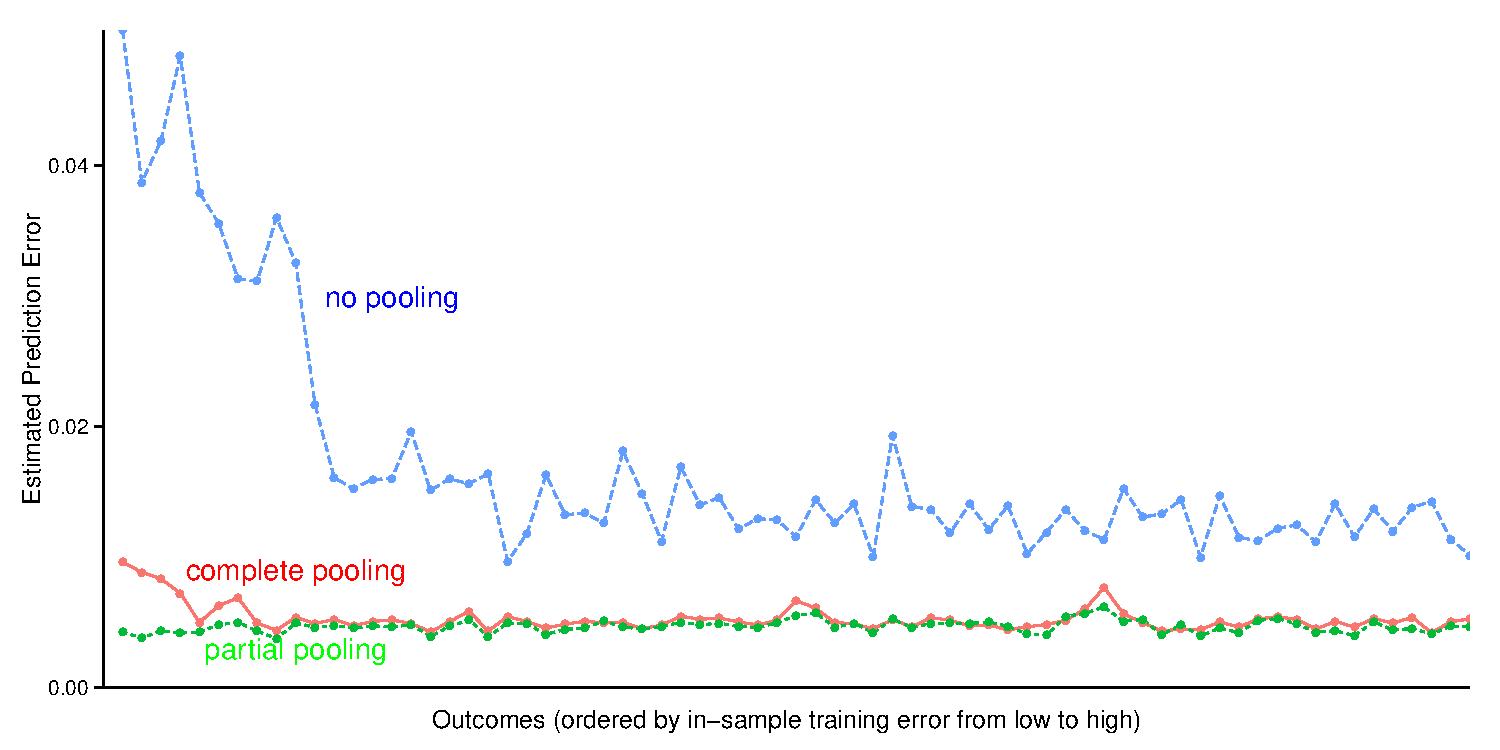
\includegraphics[width=\textwidth]{alloutcomesx1.pdf}
  \caption{\em Measure of fit (estimated prediction error) for all response outcomes
    in the 2006 Cooperative Congressional Election Survey. Outcomes are ordered by the lower bound
    (in-sample loss of the saturated model). The no pooling model
    gives a bad fit.  Partial pooling does best but in most cases is almost indistinguishable from complete pooling under the cross-validation criterion.}
  \label{fig:figx1}
\end{figure*}

I begin by estimating the prediction errors of all outcomes in the
survey. The results are shown in Figure\textasciitilde{}\ref{fig:figx1}.
The \(x\)-axis is ordered by the in-sample training loss of the
saturated model \(TL(M_{\text{s}},D)\), which I use as a surrogate for a
lower bound of predictive loss. For complete pooling and partial
pooling, the prediction error stays stable across different outcomes,
while the no pooling model has huge prediction error for outcomes with
small lower bounds. This finding makes sense since these are the
settings where overfitting is most severe (saturated models achieve the
lowest in-sample training error). However, the difference in prediction
error between complete pooling and partial pooling seems negligible.
Partial pooling is giving essentially the same result as complete
pooling, at least according to cross-validation on individual survey
responses.

\begin{figure*}[p!]
  \centering
  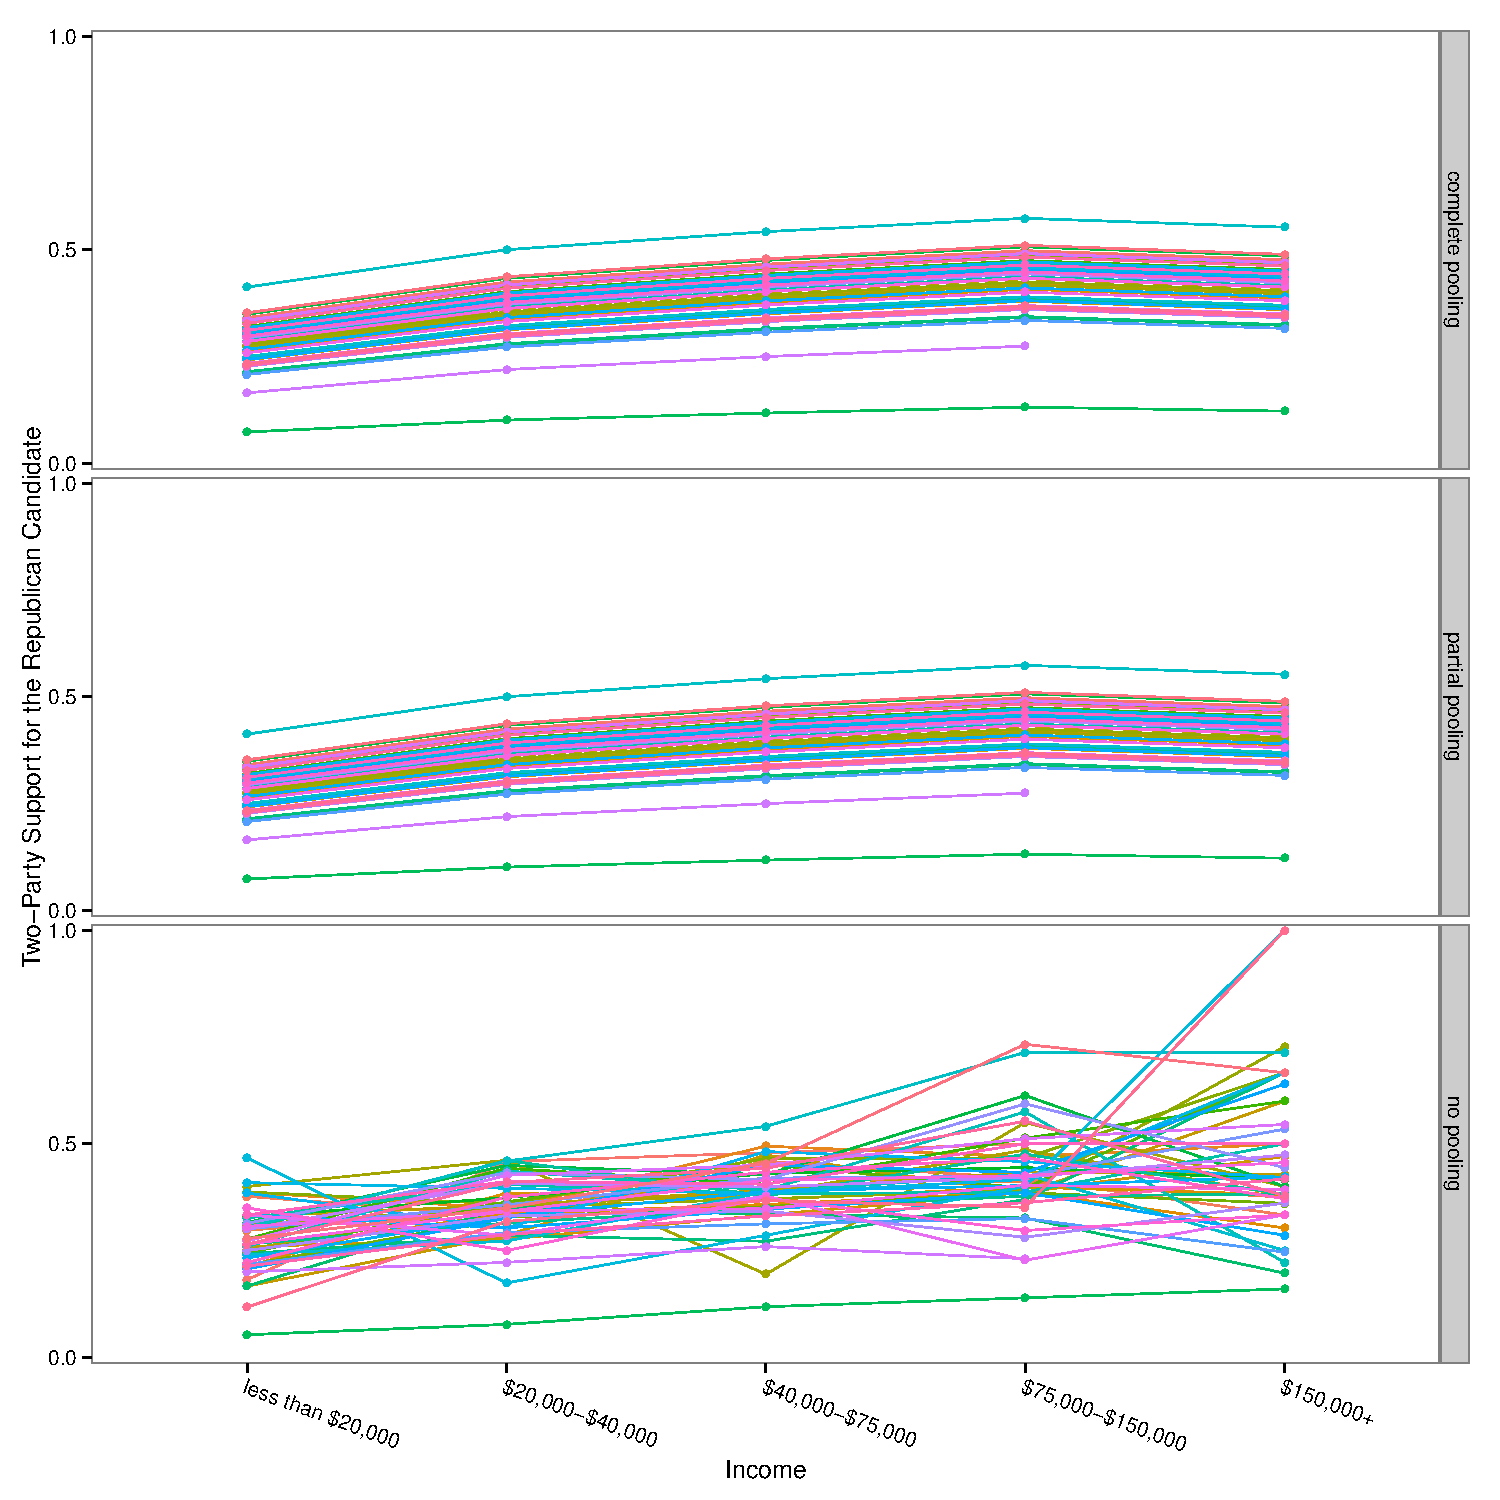
\includegraphics[width=.5\textwidth]{esti_all_bglmer}
  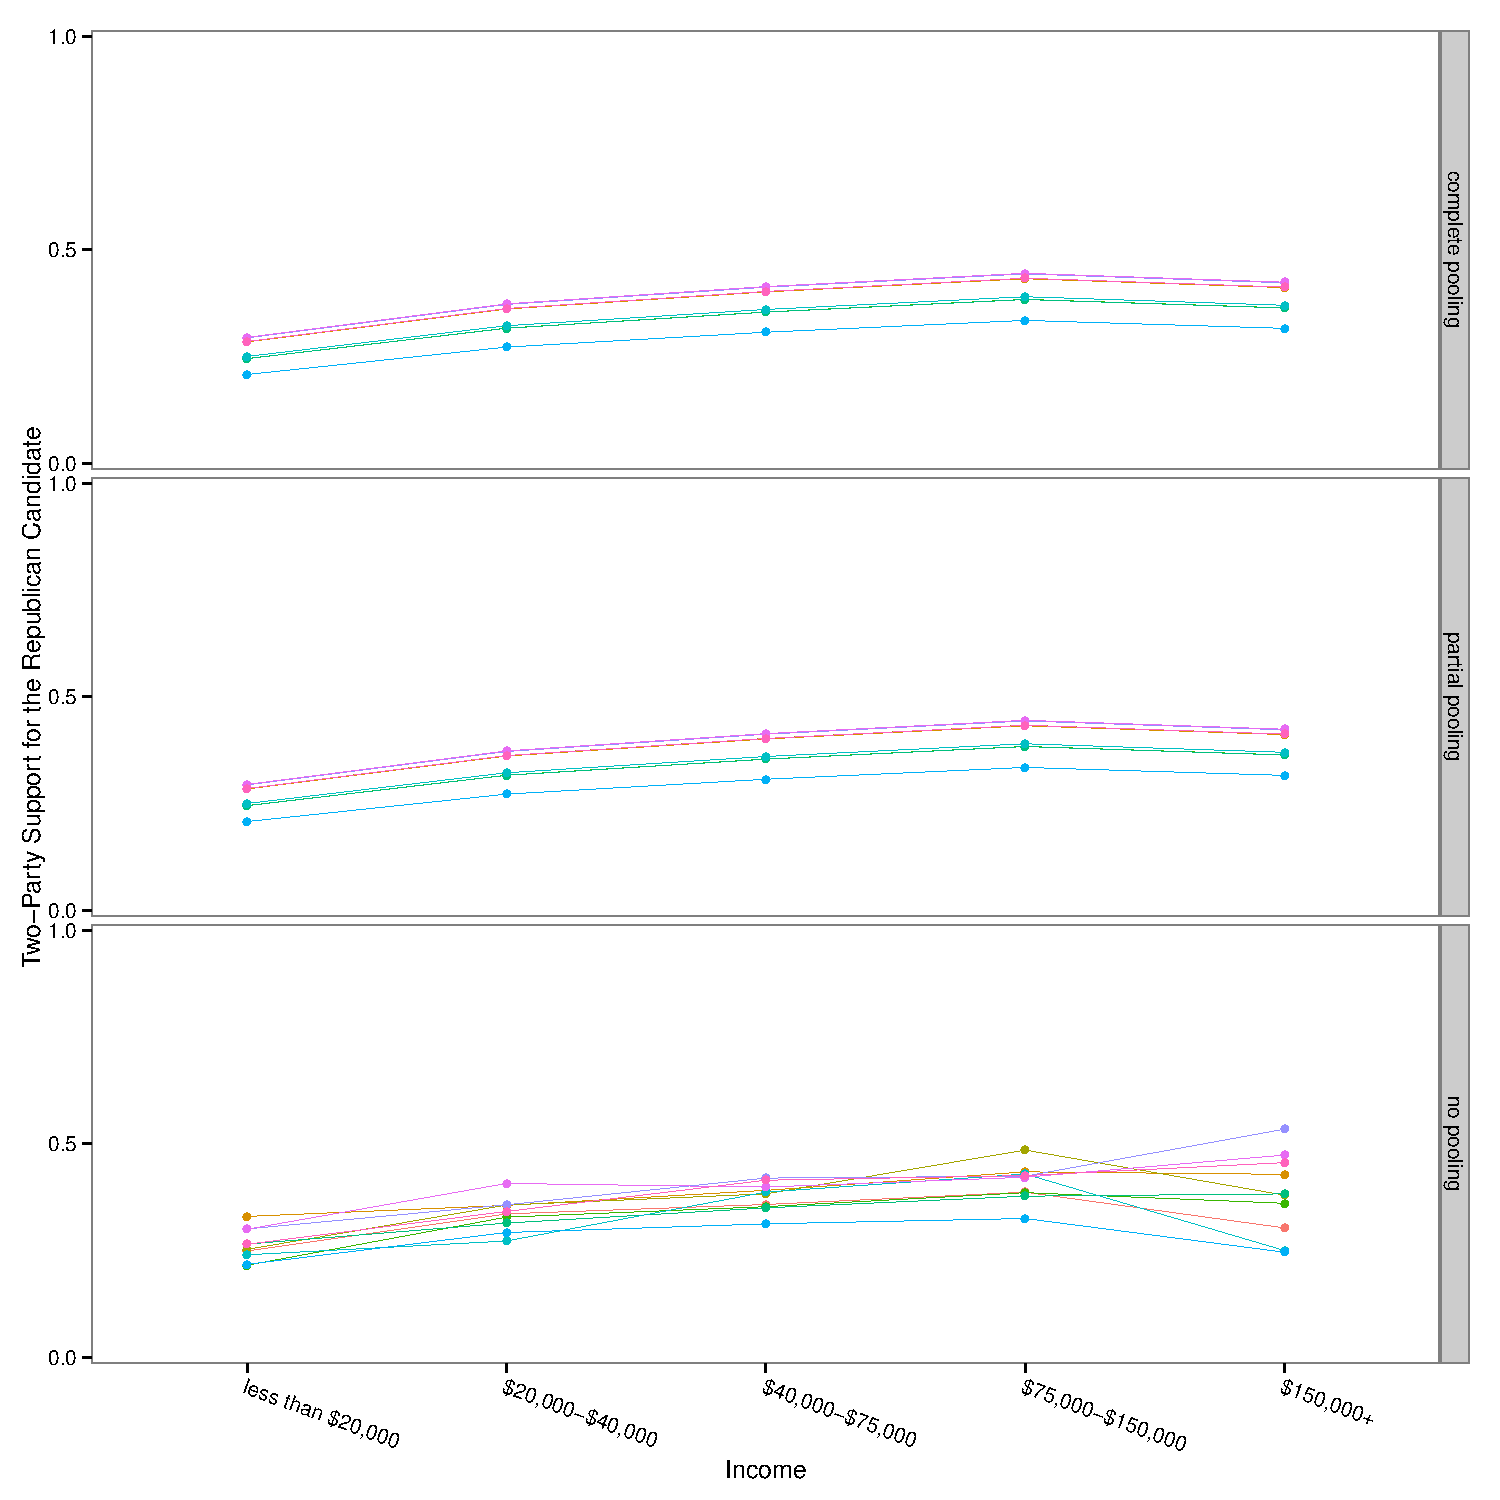
\includegraphics[width=.5\textwidth]{esti_big_bglmer}
  \caption{\em Left panel: Cell proportion estimates for three models of vote
    intention. Each line is a state. The
    partial pooling model pools so much that it is indistinguishable from
    complete pooling. Right panel: The same estimates for the 10 most populous
    states. Still, partial pooling estimates are similar to complete pooling
    estimates.}
  \label{fig:234}
\end{figure*}

This seems to suggest that partial pooling does not have enough
information to estimate cell-to-cell variation, thus giving an overly
conservative estimate. Indeed, when I plot the estimates of
\(\pi_{j_1j_2}\) for one particular outcome, vote preference for in the
congressional election (see the left panel of
Figure\textasciitilde{}\ref{fig:234}), the estimates from partial
pooling are almost identical to those from complete pooling. Even for
populous states where, because of their large sample size, the amount of
partial pooling should be small, there are no major differences between
estimates from partial pooling model and estimates from complete pooling
model (see the right panel of Figure\textasciitilde{}\ref{fig:234}).
This pattern is consistent across different outcomes.

Although partial pooling is intrinsically better than complete
pooling, it seems that the given data are not sufficient for the partial
pooling model to pick up the interaction and unpool the estimates
appropriately. It is a result of the particular characteristics of this
data set? There are three factors determining the structure of the data
that might affect the extent of pooling of the model. First is the
sample size. If I increase the sample size to a sufficiently large
level, the partial pooling model will be able to partially pool the
estimates to an appropriate amount. As sample size grows, the no pooling
model will eventually have the same performance as partial pooling, and
it might be interesting to see at what point the saturated model becomes
acceptable. The second factor affecting the relative performance of the
different models is the size of the interactions that are being
estimated, and the third factor is the level of imbalance in the
hierarchical structure. Survey data classified by demographic and
geographic predictors are typically highly unbalanced due to the long
tails of sizes typical in taxonomic structures (Mandelbrot 1955). For
example, the 2006 CCES includes 3,637 respondents from California but
only 131 from Arkansas. This unbalanced structure will affect the amount
of pooling performed by a multilevel model.

In the following subsections, I conduct simulations that vary sample
size and the structure of the cells to investigate how these factors
affect the relative performance of the three models as captured by
cross-validation.

\subsection{How Sample Size Changes the
Dynamics}\label{how-sample-size-changes-the-dynamics}

\begin{figure}[p!]
  \centering
  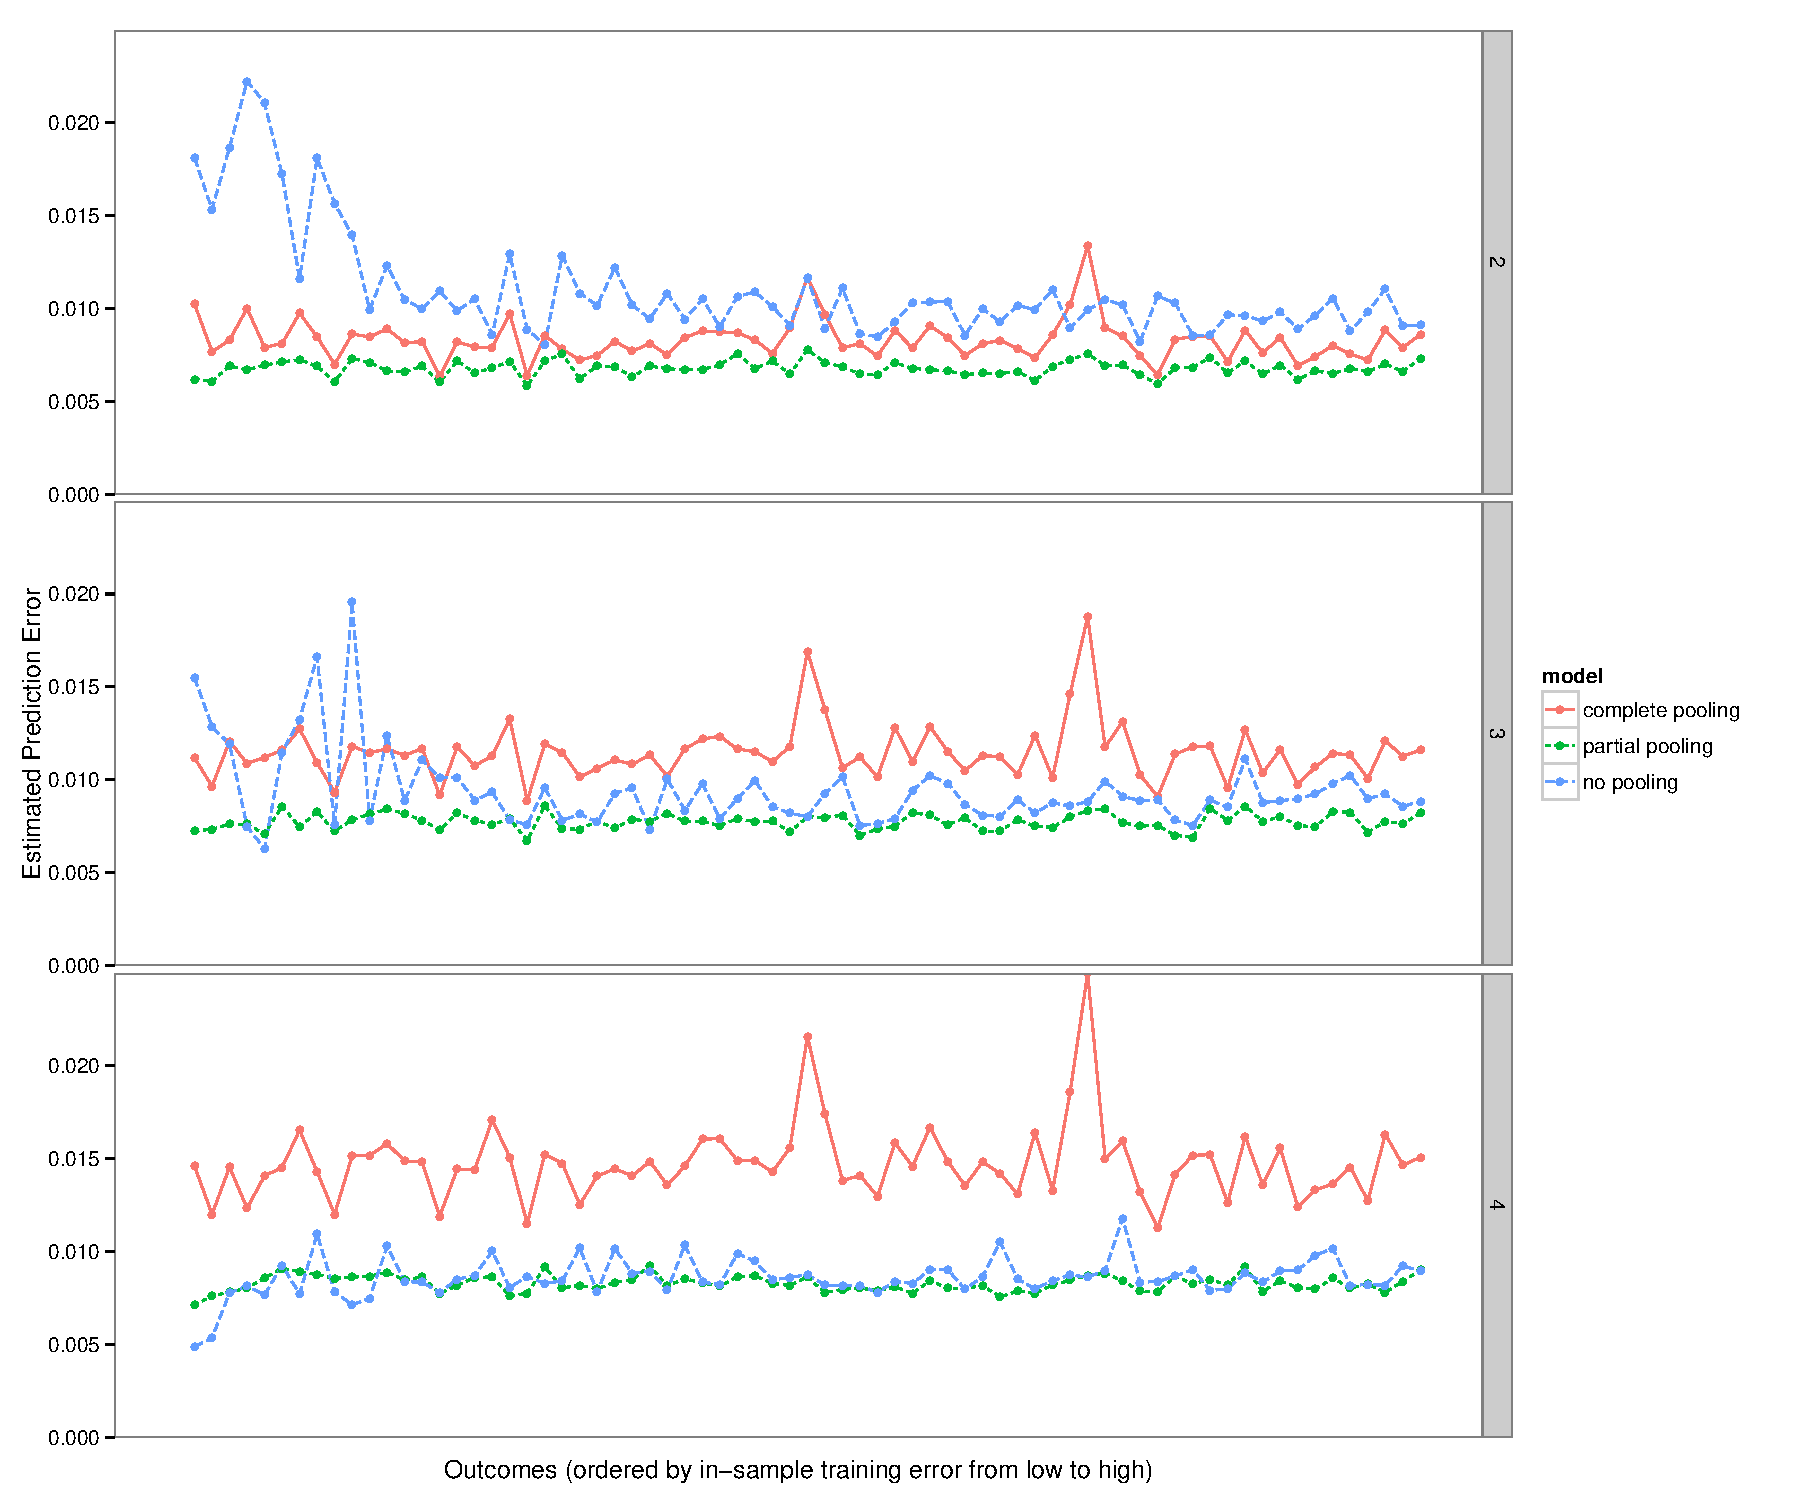
\includegraphics[width=\textwidth]{outcome234.pdf}
  \caption{\em Estimated prediction error of all response outcomes for augmented
    data sets. From top to bottom, the data sets have 2, 3, and 4 times as many
    data points as the original data set. The outcomes are ordered by the
    in-sample predictive loss. As sample size grows, complete pooling
    gradually gets worse and no pooling gets better.}
  \label{fig:figx234}
  \end{figure}

I artificially augment the data set by combining the data set with
itself. New data sets with sample size that are 2, 3 and 4 times as
large are generated. This augmentation still maintains the same level of
interactions and cell structure as those of the original data. Then I
estimate the prediction errors for all outcomes for the three models.
Results are plotted in Figure\textasciitilde{}\ref{fig:figx234}. As I
expected, as sample size grows, the prediction error of complete pooling
model, which is essentially a wrong model, dominates the other two;
while the prediction error of no pooling model keeps decreasing. When
the sample size is 4 times as large as the original data set, no pooling
model has almost the same prediction error as partial pooling model.
This makes sense, since the problem of overfitting eventual goes away if
there are sufficiently large sample size and fixed model structure.

\begin{figure*}[p!]
  \centering
  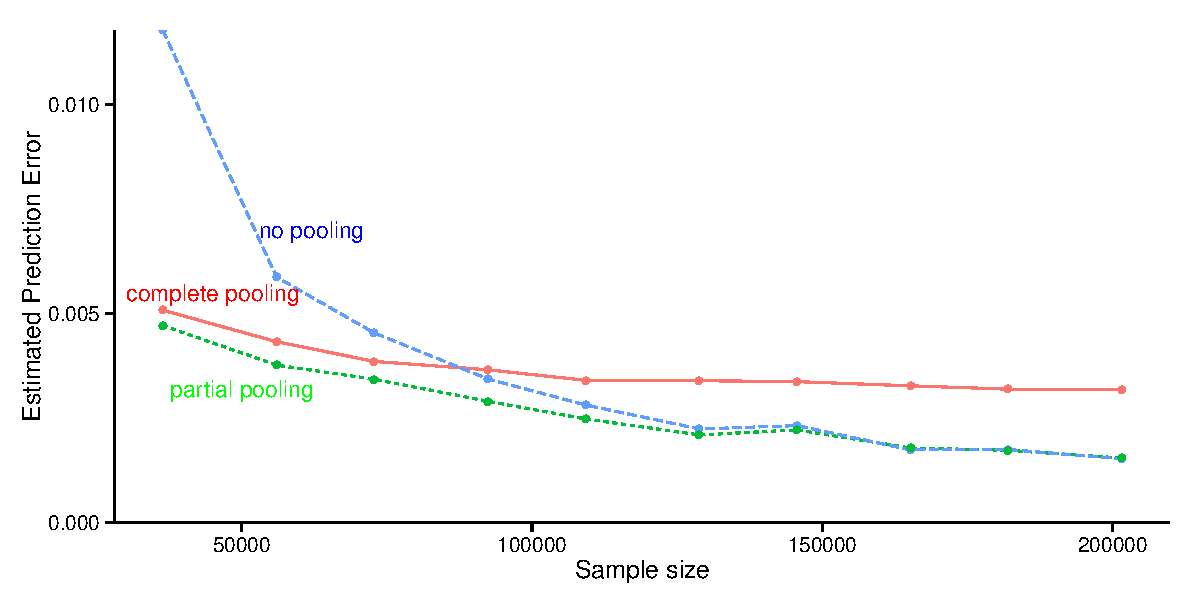
\includegraphics[width=\textwidth]{hourvote.pdf}
  \caption{\em Prediction error of the three models as sample size grows. The
    outcome under consideration is partisan vote preference in the upcoming
    congressional election. By this criterion, partial pooling and complete
    pooling perform similarly until sample size exceeds 50,000.}
  \label{fig:hourvote}
\end{figure*}

These results suggest that for a fixed data structure, partial pooling
decisively outperforms no pooling and complete pooling only for a
certain window of sample sizes. To have a closer look at the range of
the window, I look at one particular outcome, the vote preference in the
upcoming election for the U.S. House of Representatives. I augment the
sample size and plot the relative performance of the three models in
Figure\textasciitilde{}\ref{fig:hourvote}. Partial pooling model is
noticeably better than complete pooling in this setup when the total
sample size exceeds larger than 50,000. Other outcomes have similar
patterns.

\subsection{Balancedness of the Hierarchical
Structure}\label{balancedness-of-the-hierarchical-structure}

One possible explanation for the steep learning curve of the partial
pooling model is the highly unbalanced structure of the data. Although
there are 50 states, the estimate of the covariance of the state random
effects might not be reliable since some of the states have small sample
sizes. To see how the balancedness of the structure affects the model, I
simulate a data set based on partial pooling estimates from the original
data set, but make each demographic-geographic cells of roughly the same
size. The overall sample size is the same as that of the real data.
Relative performance of the three models for all outcomes is plotted in
Figure\textasciitilde{}\ref{fig:figbal}. The graph shows that with
balanced hierarchical structure, at the same sample size and amount of
interaction, partial pooling kicks in much more quickly. Thus partial
pooling is consistently better than complete pooling in this scenario.
As in the previous analysis, I also look at the relative performance of
the three models as sample size grows. The results are plotted in
Figure\textasciitilde{}\ref{fig:hourvote_bal}.

\begin{figure}[p!]
  \centering
  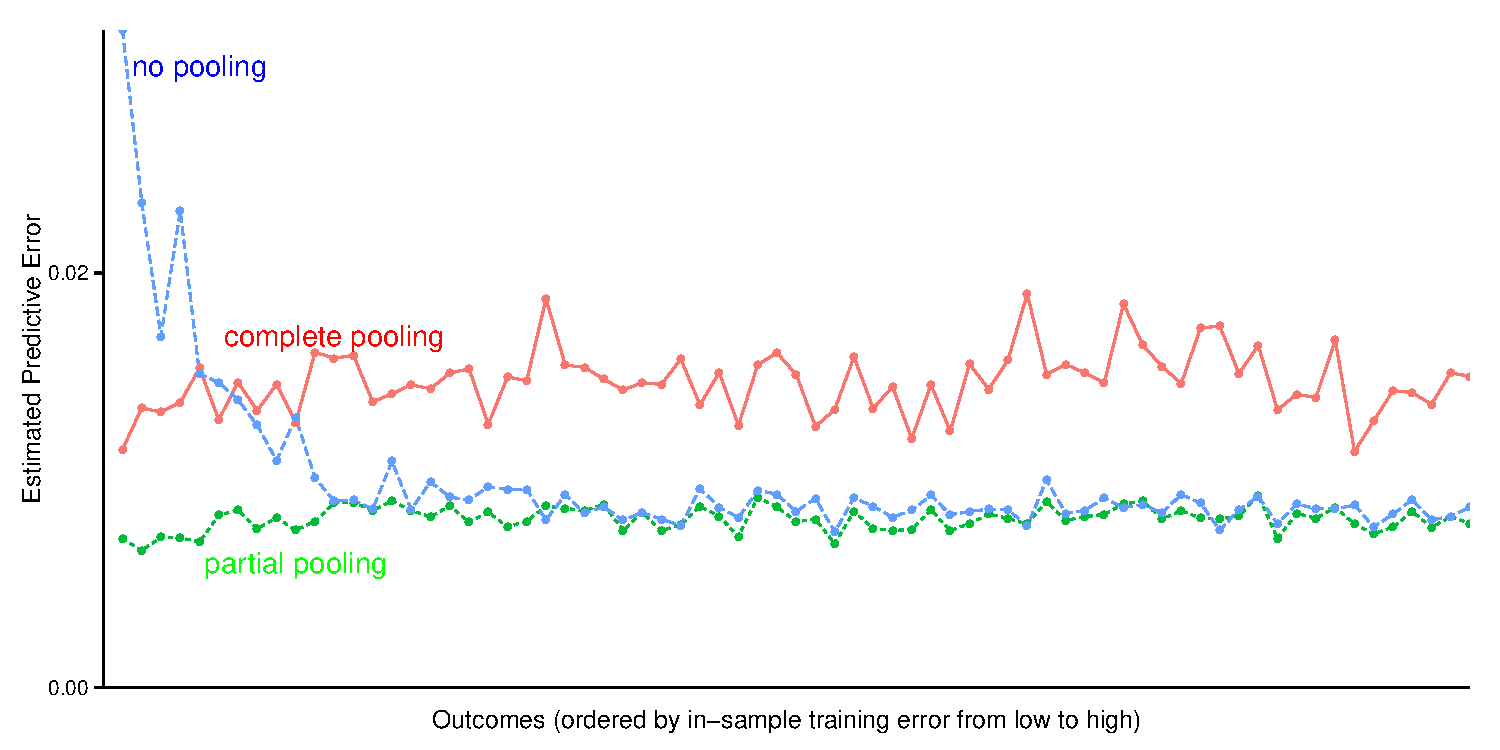
\includegraphics[width=\textwidth]{alloutcomesxbal.pdf}
  \caption{\em Measure of fit (prediction error) for all outcomes, ordered by
    in-sample training loss. The data set is simulated from real data set, and
    has the same sample size in total as the real data set, but keeping all
    demographic-geographic cells balanced. In this case, complete pooling model
    has much higher prediction errors than no pooling and partial
    pooling. Partial pooling is slightly but consistently better than no
    pooling. In particular, no pooling model has huge prediction error for
    outcomes that have smaller in-sample training loss.}
  \label{fig:figbal}
\end{figure}

\begin{figure}[p!]
  \centering
  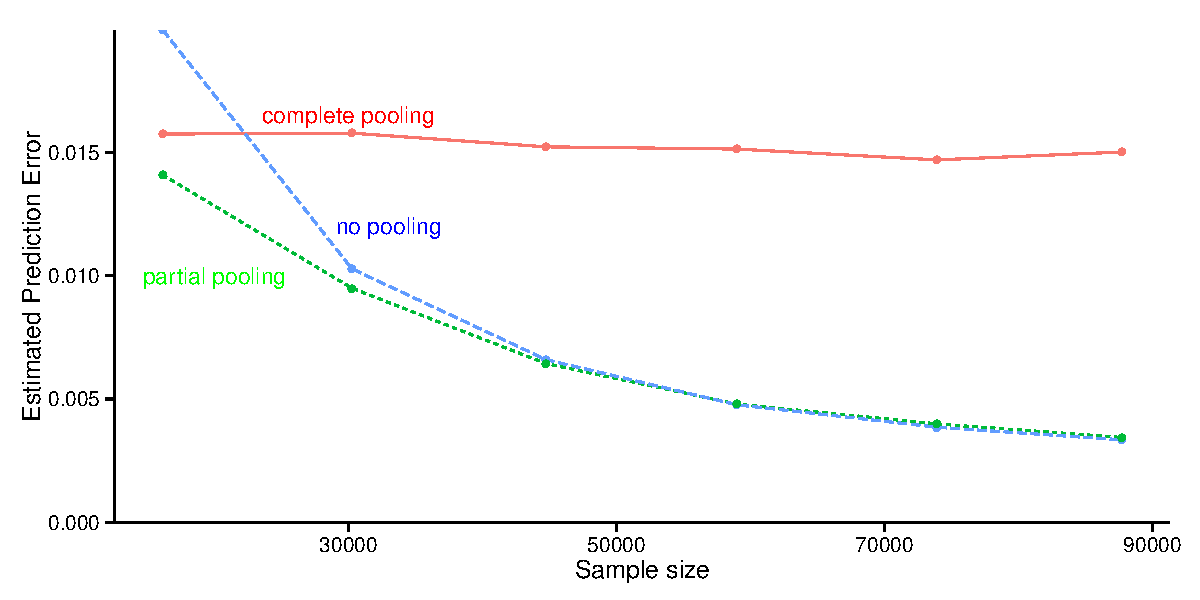
\includegraphics[width=\textwidth]{hourvote_bal.pdf}
  \caption{\em Prediction error of the three models as sample size grows under the
    simulated balanced data set. The outcome under consideration is the vote for
    the Republican candidate in the U.S House of Representatives. Partial
    pooling has the lowest prediction error when sample size is under 70,000.}
  \label{fig:hourvote_bal}
\end{figure}

\section{Discussion}\label{discussion}

Cross-validation is an important tool used to evaluate a wide variety of
statistical methods and has been widely used in model comparison when
predictive power is of concern. Some theoretical treatments have pointed
out situations where cross-validation might have problems. For example,
(Shao 1993) shows that, under the frequentist setting, using
leave-one-out cross-validation for linear model variable selection is
not consistent. However, the simplicity and transparency of
cross-validation gives it a near-universal appeal. In this paper, I
investigate the sensitivity of cross-validation as a model comparison
instrument in a cross-tabulated multilevel survey data set.

I set up the model selection problem, considering three models for these
structured data: the classical models of complete pooling and no
pooling, and a Bayesian multilevel model. The multilevel model captures
important interactions that are not included in the complete pooling
model, while at the same time avoiding the inevitable overfitting from
the no pooling model. However, the improvement of the multilevel model
as given by cross-validation is surprisingly tiny, almost negligible to
unsuspecting eyes. The problem is that improved fits with binary data
yield minuscule improvements in log loss, in moderate sample sizes
nearly indistinguishable from noise even if the improved estimates are
substantively important when aggregated (for example, state-level public
opinion). Simulations based on real data show that sample size and
structure of the cross-tabulated cells play important roles in the
relative margins of different models in cross-validation based model
selection. Caution should be exercised in applying prediction error for
model selection with structured data.

\newpage

\hyperdef{}{references}{\label{references}}
\section*{Bibliography}\label{bibliography}
\addcontentsline{toc}{section}{Bibliography}

\hyperdef{}{ref-lme4}{\label{ref-lme4}}
Bates, Douglas, Martin Maechler, and Ben Bolker. 2013. \emph{Lme4:
Linear mixed-effects models using s4 classes}.
\url{http://CRAN.R-project.org/package=lme4}.

\hyperdef{}{ref-burman1989comparative}{\label{ref-burman1989comparative}}
Burman, Prabir. 1989. ``A comparative study of ordinary
cross-validation, v-fold cross-validation and the repeated
learning-testing methods.'' \emph{Biometrika} 76(3): 503--514.

\hyperdef{}{ref-burman1994cross}{\label{ref-burman1994cross}}
Burman, Prabir, Edmond Chow, and Deborah Nolan. 1994. ``A
cross-validatory method for dependent data.'' \emph{Biometrika} 81(2):
351--358.

\hyperdef{}{ref-butticeux5f2013}{\label{ref-butticeux5f2013}}
Buttice, Matthew K., and Benjamin Highton. 2013. ``How does multilevel
regression and poststratification perform with conventional national
surveys?'' \emph{Political Analysis} 21(4): 449--467.

\hyperdef{}{ref-chung2013nondegenerate}{\label{ref-chung2013nondegenerate}}
Chung, Yeojin et al. 2013. ``A nondegenerate penalized likelihood
estimator for variance parameters in multilevel models.''
\emph{Psychometrika} 78(4): 685--709.

\hyperdef{}{ref-craven1978smoothing}{\label{ref-craven1978smoothing}}
Craven, Peter, and Grace Wahba. 1978. ``Smoothing noisy data with spline
functions.'' \emph{Numerische Mathematik} 31(4): 377--403.

\hyperdef{}{ref-blme}{\label{ref-blme}}
Dorie, Vincent. 2013. \emph{Blme: Bayesian linear mixed-effects models}.
\url{http://CRAN.R-project.org/package=blme}.

\hyperdef{}{ref-FayHerriot:1979}{\label{ref-FayHerriot:1979}}
Fay, R. E., and R. A. Herriot. 1979. ``Estimates of income for small
places: An application of james-stein procedures to census data.''
\emph{Journal of the American Statistical Association} 74: 269--277.

\hyperdef{}{ref-gelman2007data}{\label{ref-gelman2007data}}
Gelman, Andrew, and Jennifer Hill. 2007. \emph{Data analysis using
regression and multilevel/Hierarchical models}. Cambridge University
Press.

\hyperdef{}{ref-redstate}{\label{ref-redstate}}
Gelman, Andrew et al. 2009. \emph{Red state, blue state, rich state,
poor state: Why americans vote the way they do, second edition}.
Princeton University Press.

\hyperdef{}{ref-ghitzaux5f2013}{\label{ref-ghitzaux5f2013}}
Ghitza, Yair, and Andrew Gelman. 2013. ``Deep interactions with MRP:
Election turnout and voting patterns among small electoral subgroups.''
\emph{American Journal of Political Science} 57(3): 762--776.

\hyperdef{}{ref-groves2004survey}{\label{ref-groves2004survey}}
Groves, Robert M. 2004. 536 \emph{Survey errors and survey costs}. John
Wiley \& Sons.

\hyperdef{}{ref-hjort2010bayesian}{\label{ref-hjort2010bayesian}}
Hjort, Nils Lid. 2010. \emph{Bayesian nonparametrics}. Cambridge
University Press.

\hyperdef{}{ref-kale2011cross}{\label{ref-kale2011cross}}
Kale, Satyen, Ravi Kumar, and Sergei Vassilvitskii. 2011.
``Cross-validation and mean-square stability.'' In \emph{Innovations in
computer science,} Tsinghua University Press, p. 487--495.

\hyperdef{}{ref-laxux5f2009}{\label{ref-laxux5f2009}}
Lax, Jeffrey R., and Justin H. Phillips. 2009. ``How should we estimate
public opinion in the states?'' \emph{American Journal of Political
Science} 53(1): 107--121.

\hyperdef{}{ref-laxux5f2013}{\label{ref-laxux5f2013}}
Lax, Jeffrey R., and Justin H. Phillips. 2013. ``How should we estimate
sub-national opinion using MRP? Preliminary findings and
recommendations.'' \emph{Presented at Midwest Political Science
Association}.

\hyperdef{}{ref-Mandelbrot:1955}{\label{ref-Mandelbrot:1955}}
Mandelbrot, B. 1955. ``On the language of taxonomy: An outline of a
`thermostatistical' theory of systems of categories with willis
(natural) structure.'' In \emph{Information theory---Third london
symposium}, ed. Colin Cherry., p. 135--145.

\hyperdef{}{ref-pan2010survey}{\label{ref-pan2010survey}}
Pan, Sinno Jialin, and Qiang Yang. 2010. ``A survey on transfer
learning.'' \emph{IEEE Transactions on Knowledge and Data Engineering}
22(10): 1345--1359.

\hyperdef{}{ref-PriceGelmanNero1996}{\label{ref-PriceGelmanNero1996}}
Price, Phillip N., Anthony V. Nero, and Andrew Gelman. 1996. ``Bayesian
prediction of mean indoor radon concentrations for minnesota counties.''
\emph{Health Physics} 71: 922--936.

\hyperdef{}{ref-ruppert2003semiparametric}{\label{ref-ruppert2003semiparametric}}
Ruppert, David, Matt P Wand, and Raymond J Carroll. 2003.
\emph{Semiparametric regression}. Cambridge University Press.

\hyperdef{}{ref-seeger2008cross}{\label{ref-seeger2008cross}}
Seeger, Matthias W. 2008. ``Cross-validation optimization for large
scale structured classification kernel methods.'' \emph{Journal of
Machine Learning Research} 9: 1147--1178.

\hyperdef{}{ref-shao1993linear}{\label{ref-shao1993linear}}
Shao, Jun. 1993. ``Linear model selection by cross-validation.''
\emph{Journal of the American statistical Association} 88(422):
486--494.

\hyperdef{}{ref-Vehtari2012a}{\label{ref-Vehtari2012a}}
Vehtari, Aki, and Janne Ojanen. 2012. ``A survey of bayesian predictive
methods for model assessment, selection and comparison.''
\emph{Statistics Surveys} 6: 142--228.

\hyperdef{}{ref-wang2014difficulty}{\label{ref-wang2014difficulty}}
Wang, Wei, and Andrew Gelman. 2014. ``Difficulty of selecting among
multilevel models using predictive accuracy.'' \emph{Statistics and Its
Interface} 7: 1--8.

\hyperdef{}{ref-wang2014forecasting}{\label{ref-wang2014forecasting}}
Wang, Wei et al. 2014. ``Forecasting elections with non-representative
polls.'' \emph{International Journal of Forecasting}.
